\documentclass[All.tex]{subfiles}
%%---------------------------%
%%---- Обычный файл      ----%
%%---------------------------%
%\sloppy
%\documentclass[14pt,a4paper,oneside]{extarticle}	% Размер основного шрифта и формата листа
%\usepackage{xltxtra}						% Используется для вывода логотипа XeLaTeX
%\usepackage{xunicode}						% Кодировка документа
%\usepackage{polyglossia}					% Загружает пакет многоязыковой верстки
%\newfontfamily\russianfont{Book Antiqua}
%%\setmainfont{Liberation Serif}						% Основной шрифт текста
%\setmainfont{Book Antiqua}
%\setdefaultlanguage{russian}				% Основной язык текста
%\setotherlanguage{english}					% Дополнительный язык текста
%\linespread{1}							% Межстрочный интервал выбран полуторным
%\usepackage[left=2.5cm,
%right=1.5cm,vmargin=2.5cm]{geometry} % Отступы по краям листа
%\bibliographystyle{ugost2008}
%
%\usepackage{xcolor}
%\usepackage{hyperref}
%% Цвета для гиперссылок
%\definecolor{linkcolor}{HTML}{359B08} % цвет ссылок
%\definecolor{urlcolor}{HTML}{799B03} % цвет гиперссылок
%\hypersetup{pdfstartview=FitH,  linkcolor=linkcolor,urlcolor=urlcolor, colorlinks=true}
%
%%---------------------------%
%%---- Пакеты расширений ----%
%%---------------------------%
%\usepackage{xcolor}
%\usepackage{hyperref}
%% Цвета для гиперссылок
%\definecolor{linkcolor}{HTML}{359B08} % цвет ссылок
%\definecolor{urlcolor}{HTML}{799B03} % цвет гиперссылок
%\hypersetup{pdfstartview=FitH,  linkcolor=linkcolor,urlcolor=urlcolor, colorlinks=true}
%
%
%\usepackage{verbatim,indentfirst}
%\usepackage{cite,enumerate,float}
%\usepackage{amsmath,amssymb,amsthm,amsfonts}
%
%%---------------------------%
%%--- Вставка иллюстраций ---%
%%---------------------------%
%\usepackage{graphicx}
%\usepackage{subfigure}
%\usepackage{fontspec}
%%\graphicspath{{Images/}}

\begin{document}
%\pagestyle{empty} %  выключаенм нумерацию
%\setcounter{page}{3}% Нумерация начинается с третьей страницы
%\renewcommand{\contentsname}{\center{Содержание}}
%\tableofcontents


	%\addcontentsline{toc}{section}{Опыт 4. Второй закон Ньютона. Две тележки}
	\section{Второй закон Ньютона. Две тележки}


\begin{figure}[H]
	\centering 		
	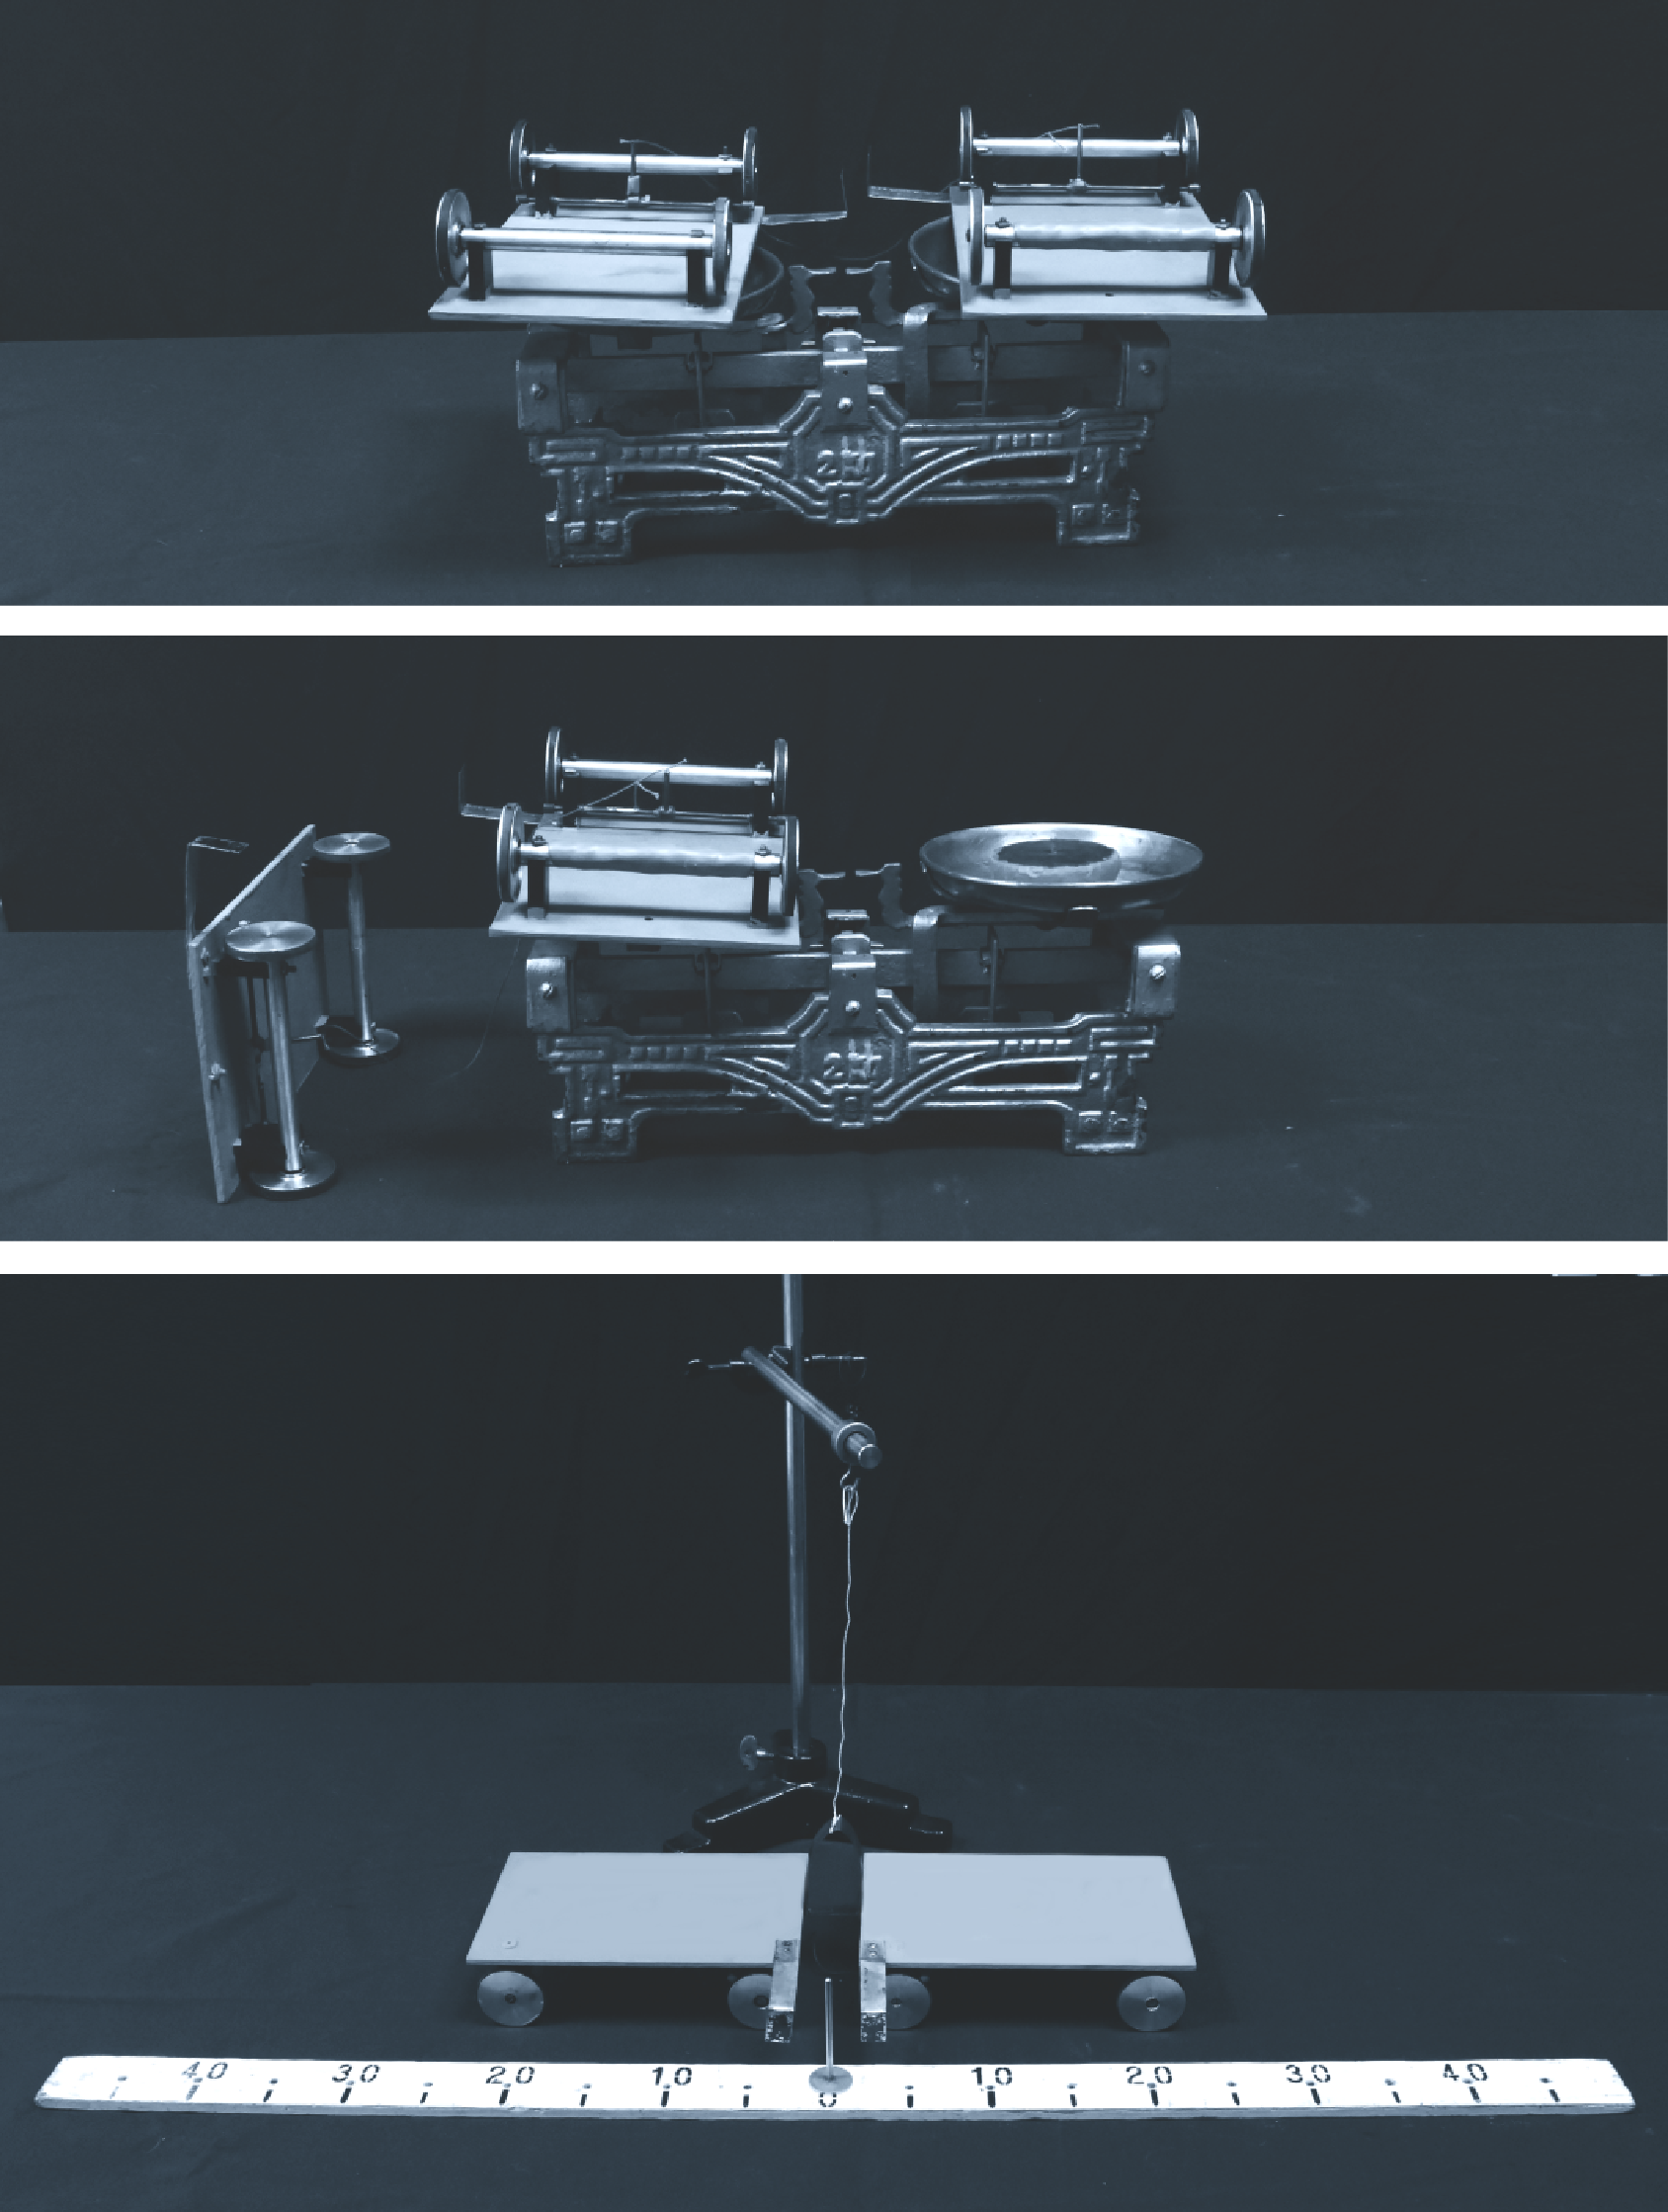
\includegraphics[width=0.6\linewidth]{newton-1.png}
	\caption{Демонстрация второго закона Ньютона}
	\label{newton-1}
\end{figure}

\subsection*{\textcolor{PineGreen}{Оборудование}}

\begin{enumerate}
	\item Пара тележек равной массы (снабженные тормозным механизмом).
	\item Штатив с подвешенной к нему тонкой стальной пластинкой.
	\item Три нитяных кольца.
	\item Метровая линейка.
	\item Груз той же массой, что и одна из тележек.
	\item Спички.
\end{enumerate}

\subsection*{\textcolor{PineGreen}{Основные определения}}

В ходе опытов можно показать, что ускорения, приобретаемые телами под действием заданной внешней силы, обратно пропорциональны массам тел: 
$$
a \sim \frac{1}{m}.
$$

Поэтому если рассмотреть два тела с массами $ m_1 $ и $ m_2 $, то значения ускорений $ a_1 $ и $ a_2 $, которые будут приобретать эти тела под действием одной и той же силы \textbf{F}, всегда будут относиться между собой как
$$
\frac{a_1}{a_2} = \frac{m_2}{m_1}.
$$

Зная связь между ускорениями и действующими силами: $ a \sim F $, а также связь между ускорением любого тела и его массой: $ a \sim 1/m$, в результате объединения этих зависимостей получится соотношение:
$$
a \sim \frac{F}{m},
$$
которое выражает физическое содержание второго закона Ньютона. 

После этого можно сформулировать второй закон Ньютона в 
следующем виде: 

\begin{flushleft}
	\textit{ускорения в движении тел прямо пропорциональны действующим 
силам и обратно пропорциональны массам движущихся тел. }
\end{flushleft}

При правильном выборе единиц формулу второго закона Ньютона 
можно записать в обеих системах (СГС или СИ) в виде простого равенства:
$$
 \textbf{a} = \frac{\textbf{F}}{m}
$$
 или
$$
\textbf{F} = m\textbf{a}.
$$
 
Здесь уже учтено, что направления ускорений совпадают с направлениями сил.
Поэтому второй закон Ньютона записан в векторной форме.

\subsection*{\textcolor{PineGreen}{Краткое описание демонстрации}}

В данной демонстрации используются две тележки на колесах одинаковой массы $m$ (рис.\ref{newton-1}).
Тележки имеют «механический» тормоз и буфер.
Перед тележками помещается демонстрационная линейка с ценой деления 10 см.
Между тележками, связанными ниткой, помещается сжатая пружина.

После пережигания нити спичкой пружина распрямляется, толкая тележки в противоположных направлениях с одинаковыми силами.
Так как изначально массы тележек равны, то пружина сообщает им одинаковые ускорения, в результате чего тележки приобретают одинаковые скорости и за равный промежуток времени перемещаются относительно начального положения на одно и то же расстояние (рис.\ref{newton-2},\textit{б}).      

\begin{figure}[H]
	\centering
	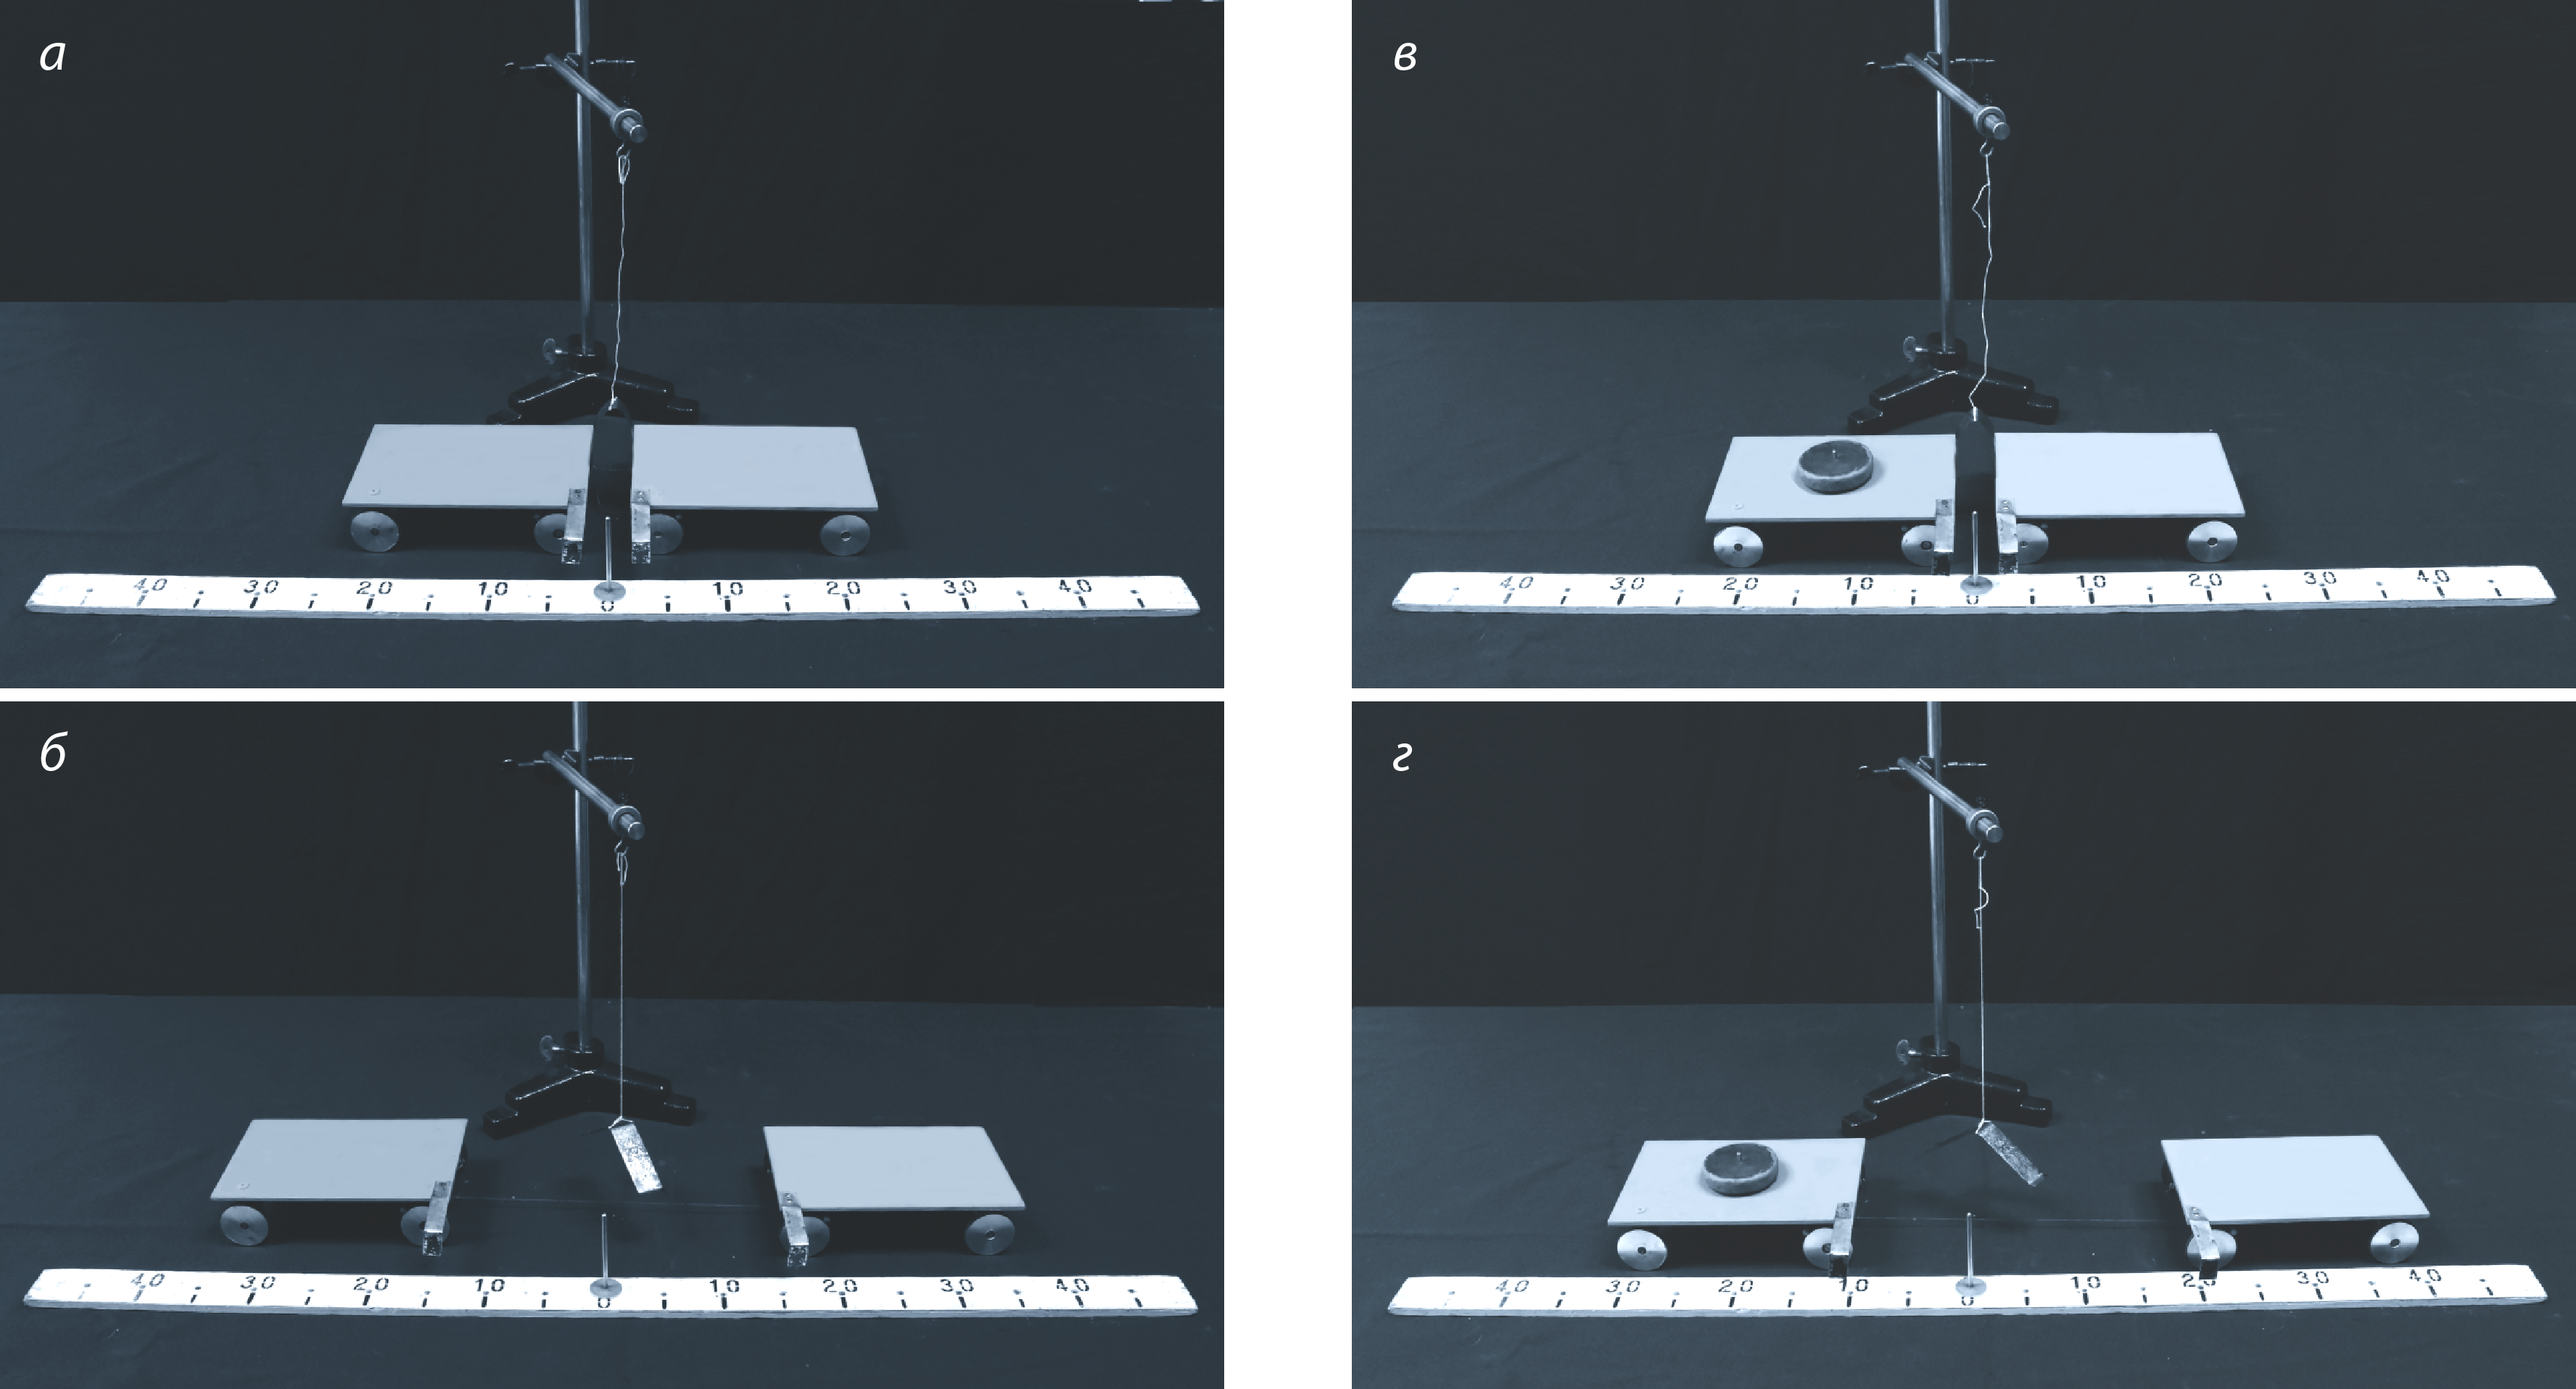
\includegraphics[width=1\linewidth]{newton-2.png}
	\caption{Демонстрация с двумя тележками: \textit{а} — начальное состояние системы, когда между тележками в сжатом состоянии располагается металлическая полоска; \textit{б} — после пережигания нити тележки равной массы разъезжаются под действием одной и той же силы на одинаковые расстояния; \textit{в,г} — при удвоении массы одной из тележек за счет дополнительного груза расстояние, которая она пройдет после пережигания нити, окажется вдвое меньше расстояния, пройденного ненагруженной тележкой}
	\label{newton-2}
\end{figure}

Если же теперь на одну тележку поместить груз массой  $ M = m $ (рис.\ref{newton-2},\textit{в}), ее масса возрастет вдвое.
После пережигания нити и распрямления металлической пластины одинаковые силы сообщат тележкам различные ускорения.
Таким образом, скорость тележки с большой массой окажется меньше скорости тележки без груза, а значит будет отличаться и пройденный путь за равные промежутки времени (рис.\ref{newton-2},\textit{г}).

\subsection*{\textcolor{PineGreen}{Теория}}

Тележки останавливаются, когда полностью натягивается нить, соединяющая рычаги тормозов. 
Следовательно, время движения каждой тележки считается одинаковым, поэтому можно записать следующее равенство:
\begin{equation}\label{newton-eq1}
 t = \frac{l}{v_{1} + v_{2}}
\end{equation}
где $ l $ — длина нити, $ v_{1} $,$ v_{2} $ — скорости тележек. 
Учитывая это соотношение, рассчитаем перемещение каждой тележки.
 \begin{equation}\label{newton-eq2}
 s_{1} = v_{1}t = \frac{v_{1}l}{v_{1} + v_{2}}, \text{   }
  s_{2} = v_{2}t = \frac{v_{2}l}{v_{1} + v_{2}}.
 \end{equation}
 Следовательно,
  \begin{equation}\label{newton-eq3}
 \frac{s_{1}}{s_{2}} = \frac{v_{1}}{v_{2}}.
 \end{equation}
 
Считая, что выпрямление зажатой пружины, которая расталкивает тележки, происходит почти мгновенно, можно воспользоваться законом сохранения импульса:
\begin{equation}\label{newton-eq4}
m_{1}v_{1} - m_{2}v_{2} = 0.
\end{equation}
Отсюда получим соотношение
\begin{equation}\label{newton-eq5}
\frac{m_{2}}{m_{1}} = \frac{v_{1}}{v_{2}}.
\end{equation}

Таким образом, пройденный тележками путь и их массы находятся в следующей зависимости:
\begin{equation}\label{newton-eq6}
\frac{s_{1}}{s_{2}} = \frac{m_{2}}{m_{1}}.
\end{equation}
В этом состоит один из способов измерения массы тела, если одну из масс принять за эталон.
Например, если $m_{1}=1$ кг, то $m_{2}=s_1/s_2$ кг).

\end{document}